To compare different codes and decoding schemes
we introduce the concept of thresholds, whereby the threshold
of a specific code of scalable distance with a specific decoding 
scheme is defined as the physical error rate $per$ at which the logical
error rate becomes greater than $50\%$ in the limit of infinite 
distance. \\
Thresholds can vary depending on the error model, i.e. 
some codes can have a higher threshold for X than for Z errors.
For simplicity's sake in the following, we will assume equal 
X, Y and Z error rates of $\frac{per}{3}$.

Using this error model, we found a threshold of $16.3\pm 0.5 \%$ for the surface code,
 $16.0\pm 0.5\%$ for the toric code and $16.1\pm0.5$ from
subfigures b), d) and f) in Figure \ref{fig:surface_threshold}.
Their thresholds are within single error margins of each other, and 
can therefore be called identical.

Since the Steane code for which we generated a lookup table is not 
a distance-scalable code, only a $pseudo$-threshold can
be found here, i.e. the crossing point to worse performance than unencoded
information. As can be seen in Figure \ref{fig: steane_threshold}, the
pseudo-threshold lies around $(1 \pm 0.5)10^{-5}$.

\begin{figure}[h!]
	\centering
	\captionsetup{justification=centering,margin=2cm}
    \subfigure[Lookup table Steane code threshold]{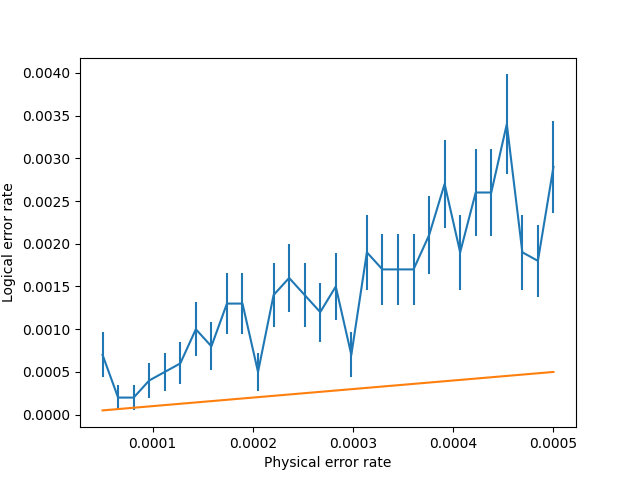
\includegraphics[width=0.4\textwidth]{./img/figures/thresholds/steaneLookupThreshold.png}}\hfill
	\subfigure[Detailed view at around $per=10^{-5}$]{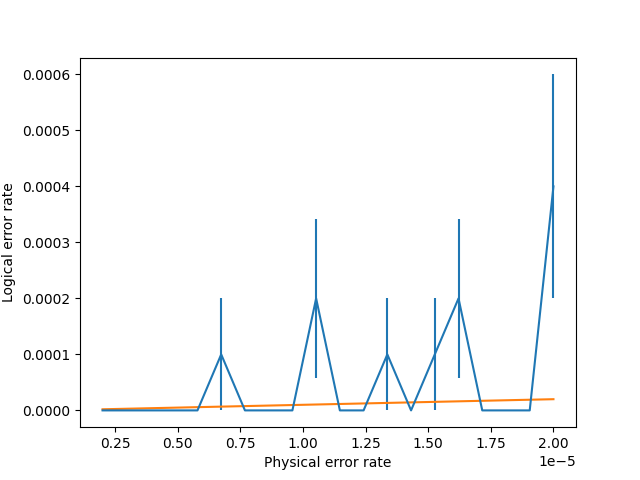
\includegraphics[width=0.4\textwidth]{./img/figures/thresholds/steaneLookupThresholdPrecise.png}}\hfill
	\caption{Lookup table pseudo threshold for the Steane code, generating code can be found in Appendix
    \ref{App: steane_thresholding}}
        
	\label{fig: steane_threshold}
\end{figure}

\begin{figure}[h!]
    \centering
    \subfigure[Surface code MWPM thresholding overview]{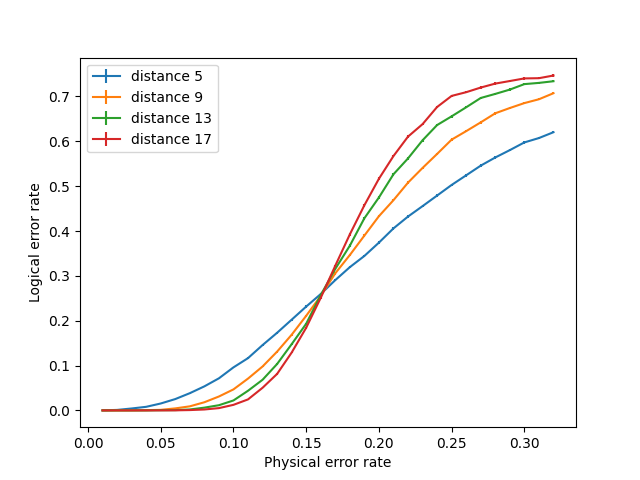
\includegraphics[width=0.4\textwidth]{img/figures/thresholds/surfaceThresholdOverview.png}}\hfill
    \subfigure[Detailed view for precise threshold determination of surface code]{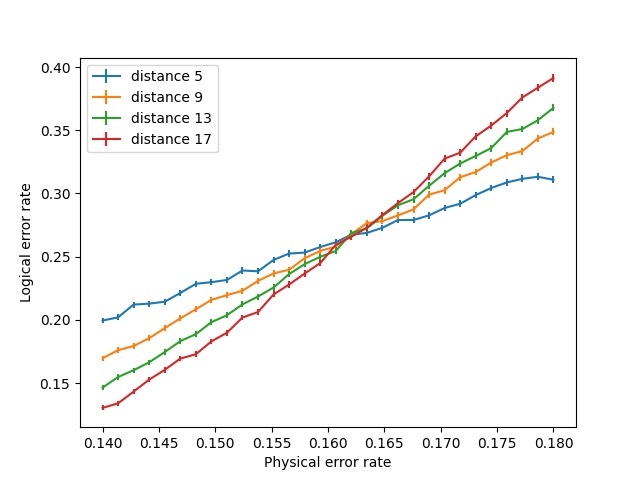
\includegraphics[width=0.4\textwidth]{img/figures/thresholds/surfaceThresholdVeryPrecise.png}}
    \subfigure[Toric code MWPM thresholding overview]{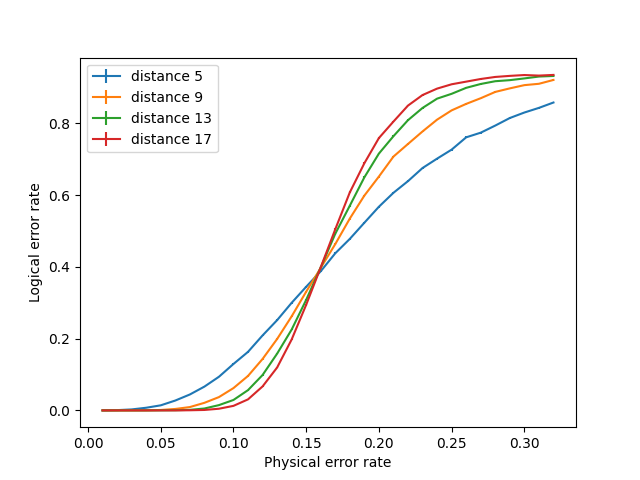
\includegraphics[width=0.4\textwidth]{img/figures/thresholds/toricThresholdOverview.png}}\hfill
    \subfigure[Detailed view for precise threshold determination of toric code]{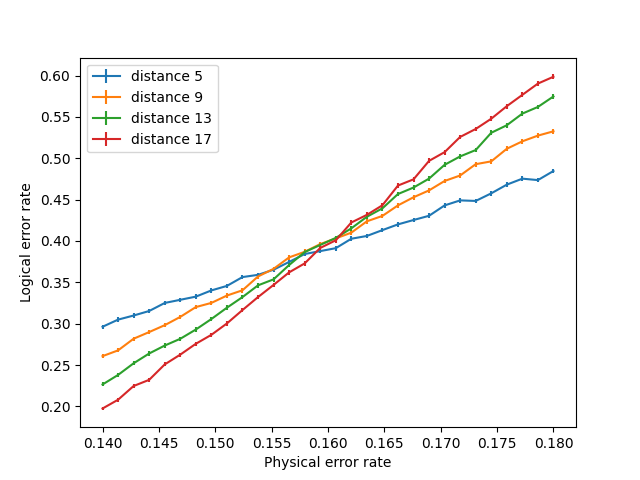
\includegraphics[width=0.4\textwidth]{img/figures/thresholds/toricThresholdVeryPrecise.png}}
    \subfigure[Cylinder code MWPM thresholding overview]{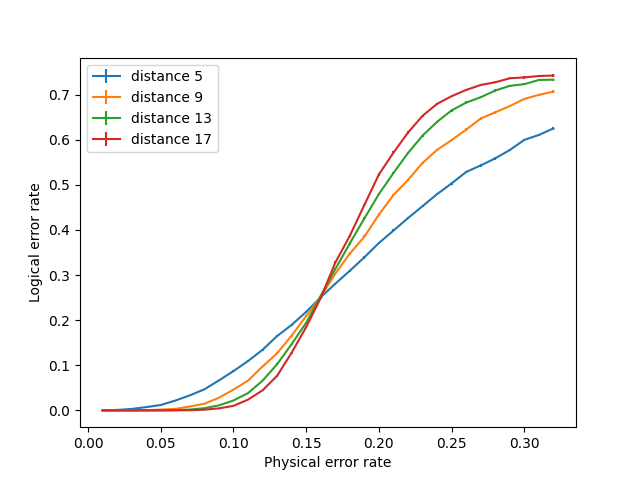
\includegraphics[width=0.4\textwidth]{img/figures/thresholds/cylinderThresholdOverview.png}}\hfill
    \subfigure[Detailed view for precise threshold determination of cylinder code]{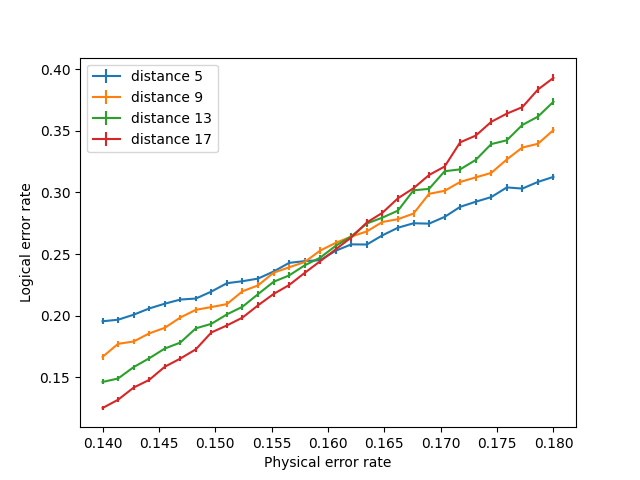
\includegraphics[width=0.4\textwidth]{img/figures/thresholds/cylinderThresholdVeryPrecise.png}}
    \caption{Thresholding of the surface/toric/cylinder code using the MWPM decoder implemented in the PyMatching \cite{MWPMDecoder} library.
    Generating code can be found in Appendix \ref{App: surface_thresholding}}
    \label{fig:surface_threshold}
\end{figure}

Unfortunately, a threshold for the hexagonal toric color code using the lifting
decoder could not be found due to a lifting bug resulting in false error predictions 
for certain error patterns.

% $c\pm b\%$ using the 
% lifting decoder for the scalable hexagonal toric color code. 
% (Reference appendix code, include a figure)
\newpage